
\documentclass[        
    a4paper,          % Tamanho da folha A4
    12pt,             % Tamanho da fonte 12pt
    chapter=TITLE,    % Todos os capitulos devem ter caixa alta
    section=Title,    % Todas as secoes devem ter caixa alta somente na primeira letra
    subsection=Title, % Todas as subsecoes devem ter caixa alta somente na primeira letra
    oneside,          % Usada para impressao em apenas uma face do papel
    english,          % Hifenizacoes em ingles
    spanish,          % Hifenizacoes em espanhol
    brazil,           % Ultimo idioma eh o idioma padrao do documento
    fleqn             % Comente esta linha se quiser centralizar as equacoes. Comente também a linha 65 abaixo
]{abntex2}

\input{lib/preambulo}

\setlength{\mathindent}{0pt} %Complementa o alinhamento de equações para totalmente a esquerda.

%%%%%%%%%%%%%%%%%%%%%%%%%%%%%%%%%%%%%%%%%%%%%%%%%%%%%
%%                     ATENCAO                     %%
%%%%%%%%%%%%%%%%%%%%%%%%%%%%%%%%%%%%%%%%%%%%%%%%%%%%%
%  Qual e o nivel do trabalho academico que voce esta 
% escrevendo? Retire o simbolo "%" apenas de um dos 
% quatro topicos abaixo refente ao nível do seu traba
% -lho.

\trabalhoacademico{tccgraduacao}
%\trabalhoacademico{tccespecializacao}
%\trabalhoacademico{dissertacao}
%\trabalhoacademico{tese}

%%%%%%%%%%%%%%%%%%%%%%%%%%%%%%%%%%%%%%%%%%%%%%%%%%%%%

% Define se o trabalho e uma qualificacao
% Coloque 'nao' para versao final do trabalho

\ehqualificacao{nao}

% Remove as bordas vermelhas e verdes do PDF gerado
% Coloque 'sim' pare remover

\removerbordasdohyperlink{sim} 

% Adiciona a cor Azul a todos os hyperlinks

\cordohyperlink{nao}

%%%%%%%%%%%%%%%%%%%%%%%%%%%%%%%%%%%%%%%%%%%%%%%%%%%%%
%%         Informacao sobre a instituicao          %%
%%%%%%%%%%%%%%%%%%%%%%%%%%%%%%%%%%%%%%%%%%%%%%%%%%%%%

\ies{Universidade Federal do Ceará}
\iessigla{UFC}
\centro{Campus Quixadá}
% \departamento{Curso de Engenharia de Software}

%%%%%%%%%%%%%%%%%%%%%%%%%%%%%%%%%%%%%%%%%%%%%%%%%%%%%
%%        Informacao para TCC de Graduacao         %%
%%%%%%%%%%%%%%%%%%%%%%%%%%%%%%%%%%%%%%%%%%%%%%%%%%%%%

\graduacaoem{Engenharia de Software}
\habilitacao{bacharel} % Ou licenciado(a)

% AVISO: Caso necessario alterar o texto de apresenta-
% cao da Especializacao, ir a pasta "lib", arquivo 
% "ufctex.sty" na linha 502.


%%%%%%%%%%%%%%%%%%%%%%%%%%%%%%%%%%%%%%%%%%%%%%%%%%%%%
%%     Informacao para TCC de Especializacao       %%
%%%%%%%%%%%%%%%%%%%%%%%%%%%%%%%%%%%%%%%%%%%%%%%%%%%%%

\especializacaoem{Yyyyyyyyy}

% AVISO: Caso necessario alterar o texto de apresenta-
% cao da Especializacao, ir a pasta "lib", arquivo 
% "ufctex.sty" na linha 507.

%%%%%%%%%%%%%%%%%%%%%%%%%%%%%%%%%%%%%%%%%%%%%%%%%%%%%
%%         Informacao para Dissertacao             %%
%%%%%%%%%%%%%%%%%%%%%%%%%%%%%%%%%%%%%%%%%%%%%%%%%%%%%

\programamestrado{Programa de Pós-Graduação em Xxxxxxx}
\nomedomestrado{Mestrado Acadêmico em Xxxxxxx}
\mestreem{Engenharia Xxxxxx}
\areadeconcentracaomestrado{Engenharia Xxxxxx}

% AVISO: Caso necessario alterar o texto de apresenta-
% cao da dissertacao, ir a pasta "lib", arquivo 
% "ufctex.sty" na linha 511.

%%%%%%%%%%%%%%%%%%%%%%%%%%%%%%%%%%%%%%%%%%%%%%%%%%%%%
%%               Informação para Tese              %%
%%%%%%%%%%%%%%%%%%%%%%%%%%%%%%%%%%%%%%%%%%%%%%%%%%%%%

\programadoutorado{Programa de Pós-Graduação em Xxxxxx}
\nomedodoutorado{Doutorado em Xxxxxxx}
\doutorem{Engenharia Xxxxxx}
\areadeconcentracaodoutorado{Engenharia Xxxxxxx}

% AVISO: Caso necessario alterar o texto de apresenta-
% cao da tese, ir a pasta "lib", arquivo "ufctex.sty" 
% na linha 515.

%%%%%%%%%%%%%%%%%%%%%%%%%%%%%%%%%%%%%%%%%%%%%%%%%%%%%
%%      Informacoes relacionadas ao trabalho       %%
%%%%%%%%%%%%%%%%%%%%%%%%%%%%%%%%%%%%%%%%%%%%%%%%%%%%%

\autor{Sávio de Carvalho Soares}
\titulo{Como a integração multidisciplinar proporciona desenvolvimento de soluções mais assertivas: Um 
estudo de caso de projeto integrado em Engenharia de Software}
\data{2026}
\local{Quixadá}

% Exemplo: \dataaprovacao{01 de Janeiro de 2012}
\dataaprovacao{}

%%%%%%%%%%%%%%%%%%%%%%%%%%%%%%%%%%%%%%%%%%%%%%%%%%%%%
%%           Informação sobre o Orientador         %%
%%%%%%%%%%%%%%%%%%%%%%%%%%%%%%%%%%%%%%%%%%%%%%%%%%%%%

\orientador{Prof. Me. Leonara de Medeiros Braz}
\orientadories{Universidade Federal do Ceará (UFC)}
\orientadorcentro{Professora Assistente}
\orientadorfeminino{sim} % Coloque 'sim' se for do sexo feminino

%%%%%%%%%%%%%%%%%%%%%%%%%%%%%%%%%%%%%%%%%%%%%%%%%%%%%
%%          Informação sobre o Coorientador        %%
%%%%%%%%%%%%%%%%%%%%%%%%%%%%%%%%%%%%%%%%%%%%%%%%%%%%%

% Deixe o nome do coorientador em branco para remover do documento

\coorientador{}
\coorientadories{Universidade Coorientador (SIGLA)}
\coorientadorcentro{Centro do Coorientador (SIGLA)}
\coorientadorfeminino{nao} % Coloque 'sim' se for do sexo feminino

%%%%%%%%%%%%%%%%%%%%%%%%%%%%%%%%%%%%%%%%%%%%%%%%%%%%%
%%              Informação sobre a banca           %%
%%%%%%%%%%%%%%%%%%%%%%%%%%%%%%%%%%%%%%%%%%%%%%%%%%%%%

% Atenção! Deixe em branco o nome do membro da banca para remover da folha de aprovacao

% Exemplo de uso:
% \membrodabancadois{Prof. Dr. Fulano de Tal}
% \membrodabancadoisies{Universidade Federal do Ceará - UFC}


\membrodabancadoisies{Universidade Federal do Ceará (UFC)}
\membrodabancadois{Prof. Dr. Jeferson Kenedy Morais Vieira}
\membrodabancatrescentro{}
\membrodabancatresies{Universidade Federal do Ceará (UFC)}
\membrodabancatres{Prof. Dra. Antonia Diana Braga Nogueira}

\begin{document}	

	% Elementos pré-textuais
	\imprimircapa
	\imprimirfolhaderosto{}
	%\imprimirerrata{elementos-pre-textuais/errata}
	\imprimirfolhadeaprovacao
	\imprimirdedicatoria{1-pre-textuais/dedicatoria}
	\imprimiragradecimentos{1-pre-textuais/agradecimentos}
	\imprimirepigrafe{1-pre-textuais/epigrafe}
	% \imprimirresumo{1-pre-textuais/resumo}
	% \imprimirabstract{1-pre-textuais/abstract}
	\renewcommand*\listfigurename{Lista de Figuras} %Se você comentar esta linha o título da lista fica: LISTA DE ILUSTRAÇÕES
	\imprimirlistadeilustracoes
	\imprimirlistadetabelas
	%\imprimirlistadequadros
	%\imprimirlistadealgoritmos
	%\imprimirlistadecodigosfonte
	% \imprimirlistadeabreviaturasesiglas
	% \imprimirlistadesimbolos{1-pre-textuais/lista-de-simbolos}   
	\imprimirsumario
	
	\setcounter{table}{0}% Deixe este comando antes da primeira tabela.
	
	%Elementos textuais
	\textual
	\chapter{Introdução}
\label{cap:introducao}

\section{O problema de Pesquisa}\label{sec:citacoes}

    Historicamente, o ensino tem sido marcado pela divisão do conhecimento em disciplinas isoladas. Isso cria uma grande distância entre o que é estudado na universidade e os desafios que o mercado de trabalho realmente exige, dificultando que os alunos percebam a utilidade prática daquilo que estão aprendendo. Oliveira (2012) explica que, por muito tempo, a educação se deparou com um grande leque de conhecimentos e de teorias valiosas, porém trabalhadas de forma desconectada. Esse modelo tradicional, muitas vezes chamado de "ensino em caixinhas", faz com que o estudante sinta que a teoria acadêmica não tem relação direta com o seu dia a dia profissional.

    Para que o desenvolvimento científico e tecnológico avance de verdade e gere um impacto positivo, é necessário superar essa separação dos saberes. Ribeiro et al. (2025) destacam que problemas reais da sociedade contemporânea raramente respeitam os limites de uma única disciplina; eles são complexos e exigem respostas que combinem várias áreas ao mesmo tempo. Nessa mesma linha, Bentes (2024) reforça que as instituições de ensino precisam modernizar seus currículos, conectando a pesquisa e a educação com a inovação, para que a universidade consiga atuar de forma prática e direta nas necessidades da comunidade. Sem essa mudança de postura, o aprendizado corre o risco de permanecer apenas na teoria.

    Diante desse cenário, onde a separação das matérias ainda é um obstáculo para a formação de bons profissionais, define-se o seguinte problema de pesquisa: \textbf{De que forma a integração multidisciplinar e interdisciplinar, aliada a metodologias ativas de ensino que estimulam o protagonismo do aluno, pode superar a fragmentação do conhecimento e impulsionar o desenvolvimento de soluções mais assertivas e inovadoras para problemas complexos?} A busca por essa resposta é o que guia o presente trabalho, exigindo uma nova visão sobre como o processo de ensino em Engenharia de Software deve ser conduzido para garantir resultados funcionais.
    
\section{A hipótese}

    A hipótese central deste trabalho é que o protagonismo do aluno proporciona a qualidade no aprendizado quando ele é inserido em um ambiente que utiliza metodologias ativas de ensino. Quando o aluno deixa de ser um mero espectador e passa a ser o construtor do próprio projeto, como no caso da Aprendizagem Baseada em Problemas (PBL), o nível de entendimento e retenção do conteúdo aumenta consideravelmente. Ao assumir a responsabilidade pela criação da solução, o estudante se sente motivado a buscar respostas em diferentes disciplinas ao mesmo tempo, quebrando de vez a barreira do ensino isolado.

    Ao substituir o isolamento das matérias por uma abordagem multidisciplinar e interdisciplinar, o processo educacional passa a refletir as reais dificuldades e a complexidade do mundo corporativo. Acredita-se que, ao permitir que o aluno interaja com múltiplas áreas do conhecimento de forma integrada (formando uma verdadeira "rede de saberes"), ele desenvolve uma maior capacidade de análise, pensamento crítico, criatividade e habilidades para trabalhar em equipe. Oliveira (2012) defende que o pensamento integrado ajuda o estudante a relacionar os conteúdos de forma sistêmica, tornando o aprendizado algo natural e útil.

    Consequentemente, essa união entre disciplinas atua como um motor essencial para o desenvolvimento de software e tecnologias. Ao trabalhar de forma colaborativa, utilizando métodos práticos de gestão e comunicação da indústria, o estudante é capacitado a desenhar e executar projetos reais. Cruz et al. (2024) evidenciam que equipes engajadas em propósitos comuns e que utilizam métodos integrados têm um desempenho superior na criação de produtos. Dessa forma, a vivência acadêmica culmina na concepção de softwares e soluções muito mais assertivas, práticas e com grande capacidade de inovação para o mercado.

\section{Objetivos}

    \textbf{Objetivo Geral:} Analisar como a integração multidisciplinar e interdisciplinar no ambiente educacional, impulsionada por metodologias ativas de ensino e pelo protagonismo do aluno, contribui para o desenvolvimento científico e proporciona a criação de soluções mais assertivas para os desafios complexos da sociedade e do mercado.

    \textbf{Objetivos Específicos:} Para que o objetivo geral desta pesquisa seja atingido de maneira estruturada, foram definidos os seguintes passos práticos, focados na avaliação das disciplinas de Projeto Integrador (PIES) do curso de Engenharia de Software na UFC (Universidade Federal do Ceará):

    \begin{itemize}
        \item \textbf{Identificar os principais desafios e barreiras} que os estudantes enfrentam em relação ao ensino dividido em disciplinas isoladas e à falta de conexão prática no início do seu aprendizado técnico.
        \item \textbf{Mapear como os conteúdos das disciplinas concomitantes} de cada semestre se unem e oferecem o suporte técnico e de negócios necessário para o bom andamento das disciplinas de Projeto Integrador (PIES 1, PIES 2 e PIES 3).
        \item \textbf{Desenvolver e aplicar formulários de pesquisa} para os alunos das disciplinas de PIES, a fim de coletar dados concretos e métricas sobre o que eles acham a respeito de usar várias áreas do conhecimento em um mesmo projeto.
        \item \textbf{Avaliar o impacto das metodologias ativas e do protagonismo estudantil} na qualidade do aprendizado, verificando se a atitude ativa e participativa do aluno ajuda a evitar o retrabalho e a acelerar o tempo de desenvolvimento do software.
        \item \textbf{Analisar, por meio dos resultados coletados,} se a união de diferentes saberes e matérias ao longo do curso resulta na entrega final de softwares e soluções tecnológicas mais precisas, funcionais e inovadoras para o cliente final.
    \end{itemize}
	\chapter{Fundamentação Teórica}
\label{cap:fundamentacao-teorica}

Para entender como a união de diferentes disciplinas ajuda a criar soluções de
software melhores e mais eficientes, é preciso apresentar a base teórica desta
pesquisa. Este capítulo discute a mudança de um modelo de ensino dividido em
matérias isoladas para uma visão integrada, a importância das metodologias
ativas para dar protagonismo ao estudante e como isso acontece na prática por
meio do Projeto Integrador no curso de Engenharia de Software.

A assertividade no desenvolvimento de software — ou seja, a capacidade de
entregar exatamente o que é necessário da melhor forma possível — não depende
apenas de saber programar. Ela depende da capacidade de fazer as diferentes
áreas "conversarem" entre si. \citeonline{silva2024processo} destacam que,
quando as barreiras entre os conhecimentos são derrubadas, as soluções criadas
se tornam muito mais funcionais e adequadas.

Nesse cenário, o protagonismo do aluno é o que garante que a integração
funcione. Como afirma \citeonline{ribeiro2025interdisciplinaridade}, quando o
estudante assume o comando do seu aprendizado e usa a interdisciplinaridade
como ferramenta, ele desenvolve um pensamento crítico que permite criar
soluções que realmente funcionam no mundo real. Portanto, integrar matérias
como banco de dados, arquitetura e testes de forma simultânea não é apenas um
método de ensino, mas a estratégia central para formar profissionais capazes de
entregar tecnologia de alta qualidade e com valor real para a sociedade.

\section{Do Ensino Dividido à Integração de Saberes: Multidisciplinaridade e Interdisciplinaridade}\label{sec:do-ensino-dividido}

Historicamente, o ensino superior foi organizado de forma muito fragmentada,
separando o conhecimento em áreas isoladas. Segundo
\citeonline{ribeiro2025interdisciplinaridade}, o ensino ainda é fortemente
dividido em disciplinas isoladas, o que faz com que os estudantes tenham
dificuldade em aplicar o conhecimento para resolver problemas reais, que são
sempre complexos e misturados. Embora esse modelo tenha ajudado a aprofundar os
estudos em áreas específicas no passado, hoje ele prejudica a formação prática.
No desenvolvimento de software, criar um aplicativo exige, ao mesmo tempo,
conhecimentos de lógica de programação, facilidade de uso, regras de negócio e
infraestrutura \cite{paulista2018desenvolvimento}.

Para resolver essa divisão, a literatura recomenda integrar as matérias, com
destaque para os conceitos de multidisciplinaridade e interdisciplinaridade. A
multidisciplinaridade acontece quando várias disciplinas trabalham em um mesmo
projeto lado a lado, mas cada uma mantém seu próprio foco. De acordo com
\cite{bentes2024integracao}, usar uma visão multidisciplinar é o que faz a
diferença na hora de criar soluções integradas para problemas complexos. Na
criação de um produto digital, equipes multidisciplinares são necessárias para
cobrir todas as partes do sistema, mesmo que às vezes enfrentam dificuldades de
comunicação por não compartilharem a mesma "língua" técnica
\cite{silva2024processo}.

Por outro lado, a interdisciplinaridade vai além e cria uma união real e
contínua entre os conhecimentos. Como definem
\citeonline[p.~10]{scherer2011interdisciplinaridade}, a interdisciplinaridade é
uma "maneira complexa de entendimento e enfrentamento dos problemas" que
integra as disciplinas através do diálogo e da negociação constante. Na prática
da sala de aula, isso significa que a escolha feita na arquitetura de um
sistema (uma disciplina) afeta diretamente a qualidade do código e a estrutura
do banco de dados (outras disciplinas). É dessa mistura que o ensino deixa de
ser apenas a transmissão de regras isoladas e se torna um espaço para o
desenvolvimento completo do aluno, preparando-o para o mercado.

Para que essa integração de matérias funcione, é preciso mudar a forma de
ensinar e de aprender. O modelo tradicional, no qual o professor apenas fala e
o aluno escuta, não serve para resolver problemas práticos que exigem
conhecimentos variados \cite{ribeiro2025interdisciplinaridade}. É aí que entram
as Metodologias Ativas, com destaque para a Aprendizagem Baseada em Problemas
(PBL) \cite{ribeiro2025interdisciplinaridade}. Essas metodologias mudam a
rotina comum da sala de aula. Para
\citeonline{ribeiro2025interdisciplinaridade}, o uso de metodologias ativas
"favorecem aprendizagens profundas e competências amplas". No ensino de
tecnologia, isso imita os desafios reais das empresas de software. Quando os
alunos recebem um problema aberto, como criar um sistema para organizar as
demandas de um cliente real, eles precisam buscar os conhecimentos de várias
matérias simultâneas para conseguir criar uma solução que funcione.

Esse esforço gera o protagonismo do estudante, que é o fator principal para um
aprendizado de qualidade, pois faz o aluno deixar de ser um espectador e passar
a ser o centro do próprio aprendizado \cite{ribeiro2025interdisciplinaridade}.
O aluno protagonista entende o motivo de estar estudando aquele assunto, pois
vê a teoria sendo aplicada na hora. Como reforça
\citeonline{bentes2024integracao}, as universidades têm o dever de formar
profissionais que saibam se adaptar e que consigam usar o que aprenderam em
diferentes situações. Assim, ao invés de aprender apenas a usar uma ferramenta,
o estudante ganha a flexibilidade necessária para inovar e criar produtos de
software realmente úteis.

Embora a Aprendizagem Baseada em Problemas seja muito conhecida, existem outros
modelos e métodos de trabalho que se alinham perfeitamente com a criação de
sistemas. A Aprendizagem Baseada em Projetos, por exemplo, exige que os alunos
construam um produto real do início ao fim
\cite{ribeiro2025interdisciplinaridade}. No contexto tecnológico, isso
significa planejar, programar e entregar um software completo e funcional ao
longo de um semestre.

Para dar conta dessa entrega, as metodologias ágeis são trazidas do mercado de
trabalho direto para a sala de aula. Os alunos se organizam em equipes de
desenvolvimento, dividem as tarefas em ciclos de entrega e gerenciam o próprio
tempo para alcançar o objetivo final do projeto. Como define
\citeonline{sutherland2019scrum} em sua obra "Scrum: a arte de fazer o dobro do
trabalho na metade do tempo", esse formato ágil permite que as equipes resolvam
problemas complexos de forma mais rápida e com foco na qualidade contínua, o
que se adapta muito bem ao ritmo e aos prazos do ambiente acadêmico.

Dentro dessas equipes, o desenvolvimento do software ocorre por meio da
aprendizagem cooperativa. De acordo com \citeonline{johnson1994learning}, para
que a cooperação exista de fato, é necessário que o sucesso do projeto dependa
do esforço mútuo e da responsabilidade de todos. Na prática, cada estudante
assume uma tarefa técnica no sistema, mas todos precisam dialogar
constantemente para que as partes do código se conectem sem erros. Quando
surgem bloqueios técnicos durante essa construção, aplica-se naturalmente a
Instrução aos Pares (Peer Instruction). Criada pelo professor
\citeonline{mazur1996peer} na década de 1990, essa abordagem foca na
participação ativa, incentivando que os próprios alunos debatam os conteúdos e
encontrem as respostas juntos. Dessa forma, um aluno que tem mais domínio sobre
a infraestrutura pode explicar um conceito para um colega focado no visual do
sistema, fortalecendo a compreensão de toda a equipe.

Além da organização humana, a assertividade técnica da solução depende de
métodos práticos de engenharia, destacando-se a prototipagem rápida e os ciclos
curtos de revisão. Antes de gastar tempo escrevendo o código definitivo, os
estudantes criam simulações visuais do sistema.
\citeonline{coutinho2006prototipagem} explica que a prototipagem rápida
funciona como uma etapa fundamental no desenvolvimento ágil para avaliar
funcionalidades complexas e validar ideias de design de forma barata e
antecipada. Trabalhando em conjunto com a prototipagem, as equipes fazem
pequenas entregas parciais para receber avaliações (feedbacks) frequentes de
professores e colegas. Esse processo contínuo garante que o grupo consiga
ajustar a lógica do software e corrigir o rumo do projeto muito antes da
apresentação final.

\section{Eixos de Integração no Desenvolvimento de Software: O papel dos Projetos Integrados (PIES)}\label{sec:eixos-de-integracao}

Os Projetos Integrados em Engenharia de Software (PIES) funcionam como o
coração do currículo, pois é neles que o aluno deixa de ver as matérias de
forma isolada e passa a aplicá-las na construção de um sistema real.
\citeonline{scherer2011interdisciplinaridade} apontam que a união de diferentes
conhecimentos ajuda o estudante a enxergar o aprendizado de um jeito mais amplo
e serve para resolver problemas práticos do dia a dia. No contexto do curso,
essa estratégia serve para quebrar a ideia de que cada disciplina é uma
"caixinha" fechada e sem conexão com as outras. Essa integração acontece de
forma progressiva ao longo do curso, dividida em três grandes etapas que
aumentam de complexidade para simular os desafios reais do mercado de trabalho.

\subsection{ PIES 1: O Alicerce do Desenvolvimento (Dados e Projeto)} \label{sec:pies-1}

No primeiro estágio do projeto integrado, os alunos começam a definir o escopo
do sistema que vão criar, focado em construir a base técnica e a estrutura
inicial do software. Nesse período, as disciplinas de Projeto Detalhado de
Software e Fundamentos de Bancos de Dados trabalham juntas e dão suporte uma à
outra. Na matéria de Projeto Detalhado, o estudante aprende regras essenciais
para organizar o código, como a separação de interesses, o encapsulamento de
informações, a coesão e o acoplamento. Essas regras garantem que o código seja
limpo e fácil de mexer no futuro. Além disso, o aluno precisa lidar com
questões práticas como o tratamento de exceções (erros no sistema), a
persistência dos dados e a programação orientada por responsabilidade,
desenhando componentes e criando interfaces seguras entre os módulos do sistema
por meio de padrões de projeto (design patterns).

Ao mesmo tempo, todo esse desenho do software precisa ser guardado em algum
lugar, e é aí que entra a disciplina de Fundamentos de Bancos de Dados. O aluno
aprende a arquitetura de um Sistema Gerenciador de Banco de Dados (SGBD) e
estuda como fazer a modelagem usando o Modelo Entidade-Relacionamento e o
Modelo Relacional. Na prática do PIES 1, o estudante traduz os diagramas de
classes que fez no projeto detalhado em tabelas reais no banco de dados,
escrevendo comandos em SQL para inserir, buscar e alterar as informações. Para
garantir que o sistema não tenha dados duplicados ou quebrados, aplicam-se
conceitos avançados de restrições de integridade e normalização de tabelas.

Como mostram \citeonline{paulista2018desenvolvimento}, quando o aluno usa a lógica de programação
junto com a modelagem de dados para resolver um problema, ele consegue
resultados muito mais precisos e corretos. A vivência prática no PIES 1 faz o
estudante entender que um bom código não funciona sozinho se o banco de dados
não estiver bem estruturado. Assim, a união dessas matérias evita erros logo no
início do desenvolvimento, garantindo que o sistema comece com uma base firme
para continuar crescendo nos semestres seguintes.

\subsection{ PIES 2: Expansão para a Web e Visão de Negócio} \label{sec:pies-2}

No segundo estágio, o projeto sai do computador local e ganha uma utilidade
prática na internet, sendo preparado diretamente para o mercado de trabalho.
Esse bloco é formado pelas disciplinas de Desenvolvimento de Software para Web,
Verificação e Validação de Software \(V\&V\) e Empreendedorismo. O papel do
Desenvolvimento Web é fazer o sistema funcionar no navegador. Para isso, os
alunos aprendem sobre a internet e seus protocolos de comunicação, além de
dominarem o uso de HTML e CSS para criar a estrutura e o visual das páginas. A
disciplina também exige o uso de design responsivo e boas práticas de
acessibilidade para que o site funcione bem em qualquer tamanho de tela. Com o
uso do JavaScript, os estudantes aplicam lógica no navegador e fazem chamadas
assíncronas, permitindo que o sistema atualize as informações na tela sem
precisar recarregar a página inteira.

Para garantir que esse sistema web funcione sem falhas e com segurança, os
alunos aplicam ao projeto as técnicas da disciplina de Verificação e Validação
\(V\&V\). Eles aprendem a fazer o planejamento e a documentação das estratégias
de teste ao longo de todo o ciclo de vida do produto. Na prática, a equipe
realiza a análise estática do código e faz revisões de software para achar
problemas antes mesmo de rodar o programa. Em seguida, criam testes de unidade,
analisam a cobertura do código e usam técnicas de teste funcional (caixa preta)
e testes de integração, garantindo que a união do front-end com o banco de
dados dê certo. Os casos de teste são criados com base nas histórias de
usuários e casos de uso desenvolvidos no projeto. O grupo também usa
ferramentas de teste automatizadas ligadas a sistemas de integração contínua,
analisa relatórios de falha, aprende a isolar defeitos por meio da depuração
(debug) e faz o acompanhamento dos problemas usando ferramentas de rastreamento
(tracking), seguindo padrões conhecidos de qualidade.

Essa maturidade técnica ganha um sentido comercial por meio do
Empreendedorismo. Os alunos aprendem sobre o perfil do empreendedor, o
desenvolvimento de habilidades de negócios e a importância das pequenas
empresas na economia. A ementa aborda temas como inovação, propriedade
intelectual, transferência de tecnologia e o papel de incubadoras e parques
tecnológicos no suporte a novas ideias. Os estudantes utilizam ferramentas de
plano de negócios para entender o mercado, avaliar fontes de financiamento e
estruturar a viabilidade financeira do software que estão criando no PIES 2. De
acordo com \citeonline{bentes2024integracao}, as universidades funcionam como
motores de inovação quando conseguem conectar o que é estudado em sala de aula
com o que a sociedade e o mercado realmente precisam, diminuindo a distância
entre teoria e a prática. Desse modo, os testes de qualidade e o
desenvolvimento web passam a valorizar o plano de negócios do grupo,
transformando um exercício escolar em um produto com real potencial de mercado.

\subsection{ PIES 3: Engenharia Avançada e Qualidade de Software} \label{sec:pies-3}

Na fase final do ciclo de projetos integrados, o nível de exigência sobe para o
padrão das grandes empresas de tecnologia, onde o foco vai além de apenas fazer
o sistema funcionar: é preciso que ele seja seguro, aguente muitos acessos,
seja fácil de gerenciar e agrade ao usuário. Esse eixo maduro reúne as
disciplinas de Arquitetura de Software, Desenvolvimento para Dispositivos
Móveis, Gerência de Projetos, User Experience (UX) e Qualidade de Software. Na
matéria de Arquitetura de Software, o aluno aprende a definir a estrutura de
alto nível do sistema e estuda diferentes estilos arquiteturais, como
arquitetura em camadas, baseada em eventos, cliente-servidor ou filtros e
tubulações (pipes-and-filters). O estudante analisa a relação de custo e
benefício entre os atributos da arquitetura, cuida de questões de hardware,
garante a reutilização de código e faz a rastreabilidade dos requisitos para
que a estrutura do software respeite o que o cliente pediu.

Essa arquitetura robusta serve de base para a disciplina de Desenvolvimento de
Software para Dispositivos Móveis. Os alunos estudam os desafios da computação
móvel e aprendem a programar para plataformas como o Android SDK, criando
interfaces e layouts específicos para celulares e tablets. Eles aprendem a
trabalhar com ciclos de vida de telas (activities e intents), serviços em
segundo plano (services), mapas, localização e o uso de sensores disponíveis
nos aparelhos, como o acelerômetro e o GPS. Para que o aplicativo seja
realmente útil e fácil de usar, aplicam-se os conceitos de User Experience
(UX). Os estudantes aprendem métodos e técnicas para conhecer o comportamento
do usuário, aplicando o design de serviços no ambiente digital para criar
fluxos de navegação que sejam agradáveis e evitem a frustração de quem está
usando o aplicativo.

Para organizar todo esse trabalho técnico e de design, a Gerência de Projetos
traz os conceitos de ciclo de vida, gestão de interessados (stakeholders) e
estratégias de seleção. Os alunos gerenciam o escopo, controlam os custos
(orçamentos) e criam cronogramas gerenciando o tempo por meio da definição e
sequenciamento de atividades. Eles aplicam metodologias ágeis de mercado, como
o Scrum \cite{sutherland2019scrum}, dividindo as tarefas em ciclos de entrega e
controlando os riscos e as comunicações da equipe de forma organizada.

Por fim, a matéria de Qualidade de Software define as métricas e os padrões que
o produto deve atingir, usando modelos conhecidos como a ISO 9126-1, o CMMI e o
MPS.BR. Os alunos fazem o planejamento e a garantia da qualidade, realizam
auditorias e inspeções no código e analisam as causas de defeitos para evitar
que eles aconteçam novamente, desenvolvendo planos de qualidade oficiais.
\citeonline{silva2024processo} defendem que o desenvolvimento de produtos
digitais exige que diferentes visões trabalhem juntas para que o resultado
final seja realmente bom para o usuário. O PIES 3 consolida essa união de
gerência, arquitetura, desenvolvimento móvel, UX e qualidade, garantindo que o
software final funcione perfeitamente tanto no computador quanto no celular,
sem retrabalho e com o alto padrão exigido pelo mercado de tecnologia.

	\chapter{Trabalhos Relacionados}
\label{cap:trabalhos-relacionados}

Este capítulo apresenta e discute pesquisas que analisam como a integração de diferentes
áreas do conhecimento contribui para a eficácia no desenvolvimento de soluções e para a
elevação da qualidade do aprendizado. O objetivo desta revisão é demonstrar que a
superação da fragmentação curricular, por meio da articulação entre saberes técnicos,
científicos e sociais, constitui um caminho estratégico para a resolução de problemas
complexos da sociedade contemporânea.

\section{A interdisciplinaridade como estratégia para a formação integral no ensino
superior - Ribeiro et al., 2025.
}\label{sec:ribeiro-2025}

O trabalho de Ribeiros e colegas (2025) discute como a união de diferentes áreas do
conhecimento ajuda na formação completa dos alunos na universidade. Os autores
explicam que, hoje em dia, o ensino ainda é muito dividido em "caixinhas" (disciplinas
isoladas), o que faz com que os estudantes tenham dificuldade de resolver problemas
reais, que são sempre complexos e misturados. Para mudar isso, o artigo defende o uso de
metodologias ativas, como a Aprendizagem Baseada em Problemas (PBL), onde o aluno
deixa de ser um espectador e passa a ser o centro do aprendizado.

A pesquisa mostra que, quando as matérias se conversam e o aluno tem um papel ativo,
ele desenvolve melhor o pensamento crítico e a capacidade de criar soluções que
realmente funcionam. Os resultados indicam que essa integração não serve apenas para
passar de ano, mas para preparar o profissional para os desafios de um mercado que exige
visão de mundo e flexibilidade.

Este estudo é uma revisão bibliográfica de natureza integrativa que analisou publicações e
documentos produzidos entre 2015 e 2025. Como resultado principal, a análise teórica
consolidou o consenso de que abordagens estritamente disciplinares são insuficientes
para a resolução de problemas complexos. O trabalho demonstra, por meio da literatura
examinada, que currículos integrados e orientados a situações reais fortalecem o
engajamento estudantil e a articulação entre ensino, pesquisa e extensão, validando o
protagonismo do aluno como o elo fundamental entre a teoria acadêmica e a entrega de
soluções assertivas na prática profissional.

\subsection{Integração de Inovação Social, Empreendedorismo, Propriedade Intelectual e
Desenvolvimento Científico: Uma Abordagem Multidisciplinar - Bentes, 2024.} \label{sec:bentes-2024}

Neste estudo, Bentes (2024) analisa a convergência entre inovação social,
empreendedorismo, propriedade intelectual e desenvolvimento científico no ambiente
universitário. O autor identifica que a fragmentação dos currículos e o isolamento entre as
disciplinas impedem que as universidades respondam de forma prática às necessidades
do mercado e da sociedade. Para fundamentar essa análise, foi realizada uma revisão
integrativa da literatura de 1996 a 2023, utilizando o papel dos Núcleos de Inovação
Tecnológica (NITs) como ponto central para observar como a gestão da propriedade
intelectual pode servir de ponte entre a pesquisa acadêmica e a criação de produtos e
serviços reais.

Os resultados indicam que a integração dessas quatro áreas permite que as instituições
de ensino superior atuem como facilitadoras de desenvolvimento econômico e social. O
estudo aponta que a gestão estratégica feita pelos NITs garante a proteção das invenções
e facilita a transferência de tecnologia para o mercado, o que viabiliza a aplicação de
soluções para problemas sociais complexos. Dessa forma, a multidisciplinaridade é
apresentada como a estratégia necessária para formar profissionais capazes de conectar
o conhecimento científico a soluções inovadoras e sustentáveis. 

Esse trabalho apresenta pontos de convergência com a presente monografia, pois ambos
defendem que a integração de diferentes saberes é o melhor caminho para preparar o
estudante para desafios reais. A diferença é que, enquanto Bentes foca mais em como a
universidade deve se organizar como instituição, esta pesquisa vai além e foca no
protagonismo do aluno, defendendo que o estudante ser o centro do próprio aprendizado
é o que garante que ele realmente aprenda com qualidade e desenvolva soluções mais
assertivas.

\subsection{Desenvolvimento de Software para Solução Numérica de Equações Polinomiais:
Uma Abordagem Interdisciplinar – Silva et. al., 2018.} \label{sec:silva-2018}

O estudo de Silva e colaboradores (2018) investiga como a multidisciplinaridade impacta o
processo de design de interfaces digitais. Os autores partem do problema de que o design
moderno exige a colaboração de profissionais de diferentes áreas (como computação,
artes e psicologia), mas que essa interação frequentemente falha devido à falta de uma
linguagem comum e processos integrados. Essa fragmentação gera soluções que não
atendem plenamente às necessidades do usuário final.

Para analisar esse cenário, os autores realizaram um estudo de caso prático envolvendo
equipes multidisciplinares no desenvolvimento de produtos digitais. A análise foi feita por
meio de observação direta e entrevistas com os envolvientes, buscando entender como a
troca de conhecimentos influenciava a qualidade do artefato final. Os resultados mostram
que a integração de saberes não ocorre de forma espontânea, ela exige métodos que
facilitem o diálogo entre as áreas. Quando essa barreira é superada, observa-se um
aumento significativo na assertividade do design, resultando em interfaces mais
acessíveis e funcionais.

O trabalho de Silva e colegas (2018) é fundamental para esta monografia por apresentar
evidências práticas de que a multidisciplinaridade é um desafio de comunicação e
processo. Ele reforça a tese de que unir diferentes visões melhora a qualidade do software.
Esta pesquisa pretende avançar ao demonstrar que o protagonismo do aluno, quando
inserido nesse contexto de integração, é o que potencializa a aprendizagem e garante a
criação de soluções tecnológicas superiores.


\begin{table}[h!]	
	\centering
	\Caption{\label{tab:comparacao-trabalho-relacionados} Comparação dos trabalhos relacionados.}	
	\UFCtab{}{
		\begin{tabular}{p{2.8cm}p{3cm}p{3cm}p{3cm}p{3cm}}
			\toprule
			\textbf{Critério} & \textbf{Ribeiro et al. (2025)} & \textbf{Bentes (2024)} & \textbf{Silva et al. (2018)} & \textbf{Esta Monografia} \\
			\midrule \midrule
			\textbf{Foco Central} & Estratégias para formação integral no ensino superior. & Integração de inovação, gestão e ciência. & Processo de design e colaboração entre áreas. & Análise de como a integração de conteúdo possibilita o protagonismo.\\
			\textbf{Objeto de estudo} & Metodologias ativas e interdisciplinaridade. & NITs e currículos de Ensino Superior. & Equipes de design e desenvolvimento digital. & Metodologias ativas e integração multidisciplinar.\\
			\textbf{Abordagem metodológica} & Revisão teórica e análise de estratégias. & Revisão integrativa de literatura. & Estudo de caso com observação e entrevistas. & Análise de estudo de caso: ArenaHub.\\
			\textbf{Integração como motor de solução} & Sim (foco no desenvolvimento humano). & Sim (soluções para desafios sociais). & Sim (criação de interfaces mais assertivas). & Sim (soluções tecnológicas e educacionais).\\
			\textbf{Protagonismo do Aluno/Sujeito} & Sim (fator chave no PBL). & Indireto (foco na formação profissional). & Parcial (foco na equipe profissional). & Sim (fator central da qualidade do ensino).\\
			\bottomrule
		\end{tabular}
	}{
	\Fonte{Elaborado pelo autor.}
} 
\end{table}
	\chapter{Metodologia}
\label{chap:metodologia}

Esta seção descreve o planejamento metodológico que será executado na segunda
etapa deste trabalho (TCC2). A pesquisa classifica-se como exploratória e
descritiva, utilizando uma abordagem mista (qualitativa e quantitativa) para
compreender a fundo o fenômeno estudado \cite{creswell2010projeto}. O objetivo
é garantir que os métodos escolhidos respondam diretamente à hipótese de que o
protagonismo do aluno e a integração de saberes geram soluções de software mais
assertivas.

\begin{figure}[h!]
	\centering
	\Caption{\label{fig:fluxo-metodologico} Etapas do Processo Metodológico.}
	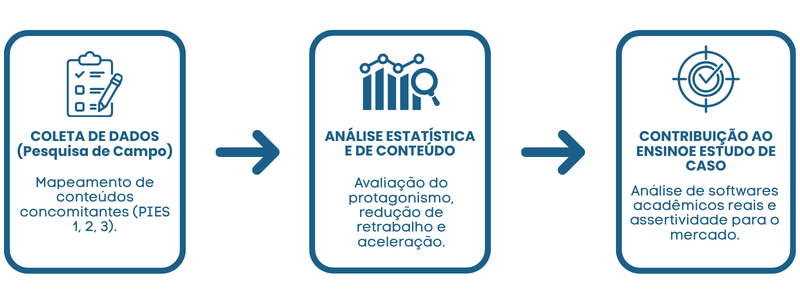
\includegraphics[width=0.9\textwidth]{figuras/metodologia_pesquisa_academica.png}
	\Fonte{Elaborado pelo autor.}
\end{figure}

Para garantir que todos os objetivos específicos sejam alcançados de forma
coerente, o processo de pesquisa foi dividido em 3 etapas sequenciais.
Esse fluxo metodológico guiará a execução do TCC2, conectando a base teórica
com a coleta e análise de dados reais.

A Figura \ref{fig:fluxo-metodologico} ilustra visualmente o fluxo dessas
etapas e resume o detalhamento técnico de cada passo que será adotado.

\newpage
\section{Coleta de Dados (Pesquisa de Campo)}\label{sec:coleta-de-dados}
Para coletar dados e métricas reais sobre a percepção dos estudantes a respeito
do uso conjunto de múltiplas áreas do conhecimento, será aplicado o método de
Survey (Pesquisa de Levantamento) \cite{gil2008metodos}.

Serão desenvolvidos três formulários digitais direcionados especificamente aos
alunos que cursam ou cursaram PIES 1, PIES 2 e PIES 3. As perguntas utilizarão
a Escala Likert de 5 pontos \cite{joshi2015likert}, permitindo quantificar o
nível de concordância dos alunos sobre o impacto das disciplinas complementares
(como Banco de Dados, Web e UX) no sucesso dos seus projetos práticos. Além
disso, o formulário conterá perguntas abertas para identificar as barreiras que
eles enfrentam com a fragmentação do ensino.

\section{Análise e Avaliação dos Resultados}\label{sec:analise-e-avaliacao-dos-resultados}
Com os dados coletados, a pesquisa passará para a etapa de análise mista. As
respostas quantitativas da Escala Likert passarão por uma Análise Estatística
Descritiva, gerando gráficos que demonstrarão o impacto das metodologias ativas
na redução do retrabalho e na aceleração do desenvolvimento. Já as respostas
abertas passarão por uma Análise de Conteúdo \cite{bardin2016analise} para
categorizar as principais dificuldades relatadas pelos estudantes.

Por fim, para analisar se a integração de diferentes saberes resultou na
entrega de softwares mais assertivos para o mercado, será utilizado o método de
Estudo de Caso \cite{yin2015estudo}. Serão selecionados projetos reais
desenvolvidos pelos alunos nas disciplinas de PIES. A avaliação focará em
cruzar as respostas dos alunos com a qualidade técnica do software entregue,
provando (ou refutando) a hipótese de que o protagonismo estudantil e a
integração de matérias geram inovação prática.
	% \chapter{Resultados}
\label{chap:resultados}

\section{Resultados do Experimento A}
\label{sec:resultados-do-experimento-a}

\section{Resultados do Experimento B}
\label{sec:resultados-do-experimento-b}

	% \input{2-textuais/6-conclusao}
	\chapter{Cronograma de Execução}
\label{sec:cronograma}


Para garantir a viabilidade e a execução estruturada da pesquisa durante o semestre letivo 
de 2026.2, foi estabelecido o cronograma apresentado na Tabela \ref{tab:cronograma-tcc2}.
As atividades dividem-se desde o refinamento dos instrumentos de coleta até a defesa pública 
do trabalho.

\begin{table}[h!]
    \centering
    \Caption{\label{tab:cronograma-tcc2} Cronograma de Atividades para 2026.2.}
    \UFCtab{}{
		\resizebox{\textwidth}{!}{
		\renewcommand{\arraystretch}{1.5}
        \begin{tabular}{p{7.5cm}cccccc}
            \toprule
            \textbf{Atividade / Etapa} & \textbf{Ago} & \textbf{Set} & \textbf{Out} & \textbf{Nov} & \textbf{Dez} \\
            \midrule \midrule
            1. Refinamento dos Questionários e Validação & X & & & & \\
            2. Aplicação do \textit{Survey} (PIES 1, 2 e 3) & X & X & & & \\
            3. Triagem e Mapeamento dos Projetos (Estudo de Caso) & & X & X & & \\
            4. Análise Estatística Descritiva (Likert) & & & X & & \\
            5. Análise de Conteúdo (Perguntas Abertas) & & & X & & \\
            6. Cruzamento de Dados e Avaliação de Assertividade & & & & X & \\
            7. Redação Final dos Capítulos de Resultados & & & & X & \\
            8. Revisão Textual e Ajustes de Formatação & & & & & X \\
            9. Entrega da Monografia e Defesa Pública & & & & & X \\
            \bottomrule
        \end{tabular}
		\renewcommand{\arraystretch}{1}
		}
    }{
        \Fonte{Elaborado pelo autor.}
    }
\end{table}


	
	%Elementos pós-textuais	
	\bibliography{3-pos-textuais/referencias}
%	\imprimirglossario	
	% \imprimirapendices
		% Adicione aqui os apendices do seu trabalho
		% \input{3-pos-textuais/apendices/apendice-a}
		% \input{3-pos-textuais/apendices/apendice-b}
		% \input{3-pos-textuais/apendices/apendice-c}
	% \imprimiranexos
		% Adicione aqui os anexos do seu trabalho
		% \input{3-pos-textuais/anexos/anexo-a}
	\imprimirindice

\end{document}